\documentclass[aspectratio=169]{beamer}
\usetheme{metropolis}
\usepackage{amsmath}
\usepackage{amssymb}
\usepackage{booktabs}
\usepackage{tikz}
\usepackage{xcolor}
\usepackage{listings}
\usetikzlibrary{arrows.meta, positioning, shapes.geometric, fit, backgrounds}

% ----- Theme tweaks -----
\definecolor{forestgreen}{HTML}{2E7D32}
\definecolor{leaf}{HTML}{66BB6A}
\definecolor{soil}{HTML}{6D4C41}
\setbeamercolor{frametitle}{bg=forestgreen, fg=white}
\setbeamercolor{progress bar}{fg=leaf, bg=leaf!30}
\setbeamercolor{title separator}{fg=leaf}
\setbeamercolor{alerted text}{fg=forestgreen}

\lstdefinestyle{mini}{
  basicstyle=\ttfamily\scriptsize,
  breaklines=true,
  showstringspaces=false,
  keywordstyle=\color{forestgreen}\bfseries,
  commentstyle=\color{soil}\itshape,
  language=Python,
}

\title{\textbf{MockingBird}}
\subtitle{A Bioacoustic Forest Health Index from a Single Audio Clip}
\author{Team Eco}
\institute{Hackathon 2026}
\date{}

\begin{document}

\maketitle

% ============================================================
\begin{frame}{Why this project?}
  \textbf{Forests are dying in ways satellites can't see.}
  \begin{itemize}
    \item NDVI and canopy cover say a forest is ``green'' --- but a green forest with no birds is an ecological corpse.
    \item Birds are the most sensitive bioindicators we have: composition shifts \alert{months to years} before vegetation collapses.
    \item Manual bird surveys are slow, expensive, and require expert ornithologists.
    \item Conservation NGOs and forest officers need \alert{a number} they can act on --- not a 200-page biodiversity report.
  \end{itemize}
  \vspace{0.6em}
  \begin{alertblock}{Our promise}
    Drop a 30-second audio clip $\rightarrow$ get a quantitative \textbf{Forest Health Quality Index (FHQI)} $\in [0,1]$ with a confidence score.
  \end{alertblock}
\end{frame}

% ============================================================
\begin{frame}{What MockingBird does --- in one slide}
  \begin{center}
  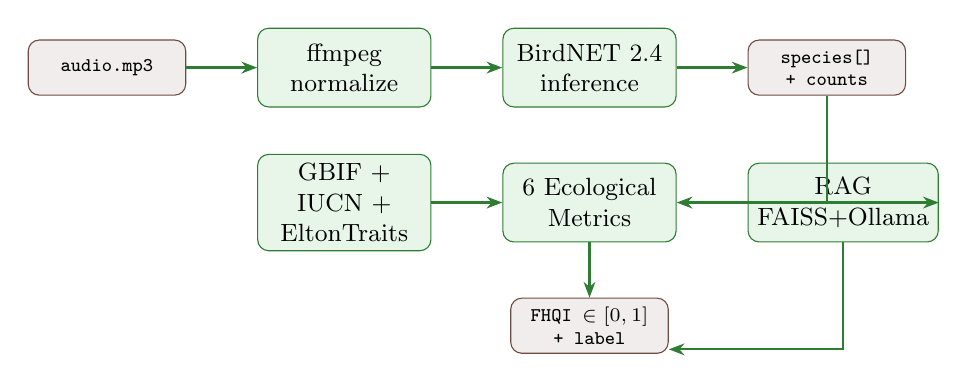
\begin{tikzpicture}[
      node distance=0.7cm and 0.9cm,
      box/.style={rectangle, draw=forestgreen, fill=leaf!15, rounded corners,
                  minimum height=1cm, minimum width=2.2cm, align=center,
                  font=\small},
      data/.style={rectangle, draw=soil, fill=soil!10, rounded corners,
                   minimum height=0.7cm, minimum width=2cm, align=center,
                   font=\scriptsize\ttfamily},
      arr/.style={-{Stealth[length=2mm]}, thick, forestgreen}
    ]
    \node[data] (audio) {audio.mp3};
    \node[box, right=of audio] (ffmpeg) {ffmpeg\\normalize};
    \node[box, right=of ffmpeg] (birdnet) {BirdNET 2.4\\inference};
    \node[data, right=of birdnet] (species) {species[]\\+ counts};
    \node[box, below=of birdnet] (metrics) {6 Ecological\\Metrics};
    \node[box, left=of metrics] (gbif) {GBIF +\\IUCN +\\EltonTraits};
    \node[box, right=of metrics] (rag) {RAG\\FAISS+Ollama};
    \node[data, below=of metrics] (fhqi) {FHQI $\in [0,1]$\\+ label};

    \draw[arr] (audio) -- (ffmpeg);
    \draw[arr] (ffmpeg) -- (birdnet);
    \draw[arr] (birdnet) -- (species);
    \draw[arr] (species.south) |- (metrics.east);
    \draw[arr] (gbif) -- (metrics);
    \draw[arr] (species.south) |- (rag.east);
    \draw[arr] (metrics) -- (fhqi);
    \draw[arr] (rag.south) |- ([yshift=-3mm]fhqi.east);
  \end{tikzpicture}
  \end{center}
  \vspace{0.3em}
  \footnotesize One endpoint $\rightarrow$ \texttt{POST /forest} returns the index, every sub-metric, and a per-species ecological profile.
\end{frame}

% ============================================================
\begin{frame}{System Architecture --- full picture}
  \begin{center}
  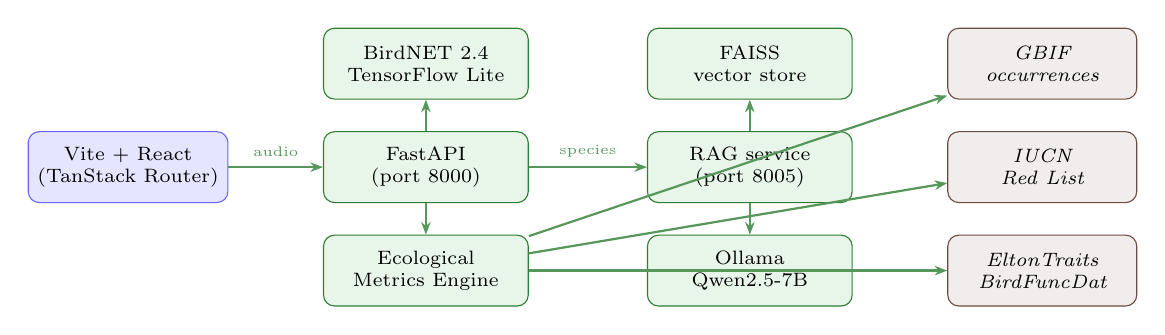
\begin{tikzpicture}[
      node distance=0.4cm and 0.5cm,
      svc/.style={rectangle, draw=forestgreen, fill=leaf!15, rounded corners,
                  minimum height=0.9cm, minimum width=2.6cm, align=center,
                  font=\scriptsize},
      ext/.style={rectangle, draw=soil, fill=soil!10, rounded corners,
                  minimum height=0.9cm, minimum width=2.4cm, align=center,
                  font=\scriptsize\itshape},
      cl/.style={rectangle, draw=blue!60, fill=blue!10, rounded corners,
                 minimum height=0.9cm, minimum width=2.4cm, align=center,
                 font=\scriptsize},
      arr/.style={-{Stealth[length=1.6mm]}, thick, forestgreen!80}
    ]
    % Client
    \node[cl] (web) {Vite + React\\(TanStack Router)};

    % Backend block
    \node[svc, right=1.2cm of web] (api) {FastAPI\\(port 8000)};
    \node[svc, above=of api] (birdnet) {BirdNET 2.4\\TensorFlow Lite};
    \node[svc, below=of api] (metrics) {Ecological\\Metrics Engine};

    % RAG
    \node[svc, right=1.5cm of api] (rag) {RAG service\\(port 8005)};
    \node[svc, above=of rag] (faiss) {FAISS\\vector store};
    \node[svc, below=of rag] (ollama) {Ollama\\Qwen2.5-7B};

    % External data
    \node[ext, right=1.2cm of faiss] (gbif) {GBIF\\occurrences};
    \node[ext, right=1.2cm of rag] (iucn) {IUCN\\Red List};
    \node[ext, right=1.2cm of ollama] (elton) {EltonTraits\\BirdFuncDat};

    \draw[arr] (web) -- node[above,font=\tiny]{audio} (api);
    \draw[arr] (api) -- (birdnet);
    \draw[arr] (api) -- (metrics);
    \draw[arr] (api) -- node[above,font=\tiny]{species} (rag);
    \draw[arr] (rag) -- (faiss);
    \draw[arr] (rag) -- (ollama);
    \draw[arr] (metrics) -- (gbif);
    \draw[arr] (metrics) -- (iucn);
    \draw[arr] (metrics) -- (elton);
  \end{tikzpicture}
  \end{center}
  \footnotesize
  \textbf{Two microservices.} Inference path (port 8000) stays hot and fast; enrichment path (port 8005) is decoupled so a slow LLM never blocks an FHQI response.
\end{frame}

% ============================================================
\begin{frame}{Tech stack \& why}
  \small
  \begin{tabular}{p{3.3cm}p{2.2cm}p{8.5cm}}
    \toprule
    \textbf{Layer} & \textbf{Tool} & \textbf{Why} \\
    \midrule
    Bird ID model        & BirdNET 2.4       & 6{,}000+ species, SOTA recall on noisy field audio, runs CPU-only \\
    API                  & FastAPI + asyncio & Native concurrency for fan-out to GBIF/IUCN/RAG \\
    Audio normalize      & ffmpeg            & Handles webm/m4a/mp3 $\rightarrow$ 48kHz mono WAV \\
    Vector DB            & FAISS (CPU)       & Local, zero-egress, sub-ms similarity search \\
    Embeddings           & all-MiniLM-L6-v2  & 384-dim, fast on CPU, strong on short biology texts \\
    LLM                  & Ollama / Qwen2.5-7B & Fully local --- no API cost, no rate limits, data stays on-prem \\
    Geocoding            & Nominatim         & Free, OSM-backed, no key required \\
    Frontend             & Vite + React + TanStack Router & File-based routing, fast HMR, type-safe params \\
    \bottomrule
  \end{tabular}
\end{frame}

% ============================================================
\begin{frame}{The audio pipeline}
  \begin{enumerate}
    \item \textbf{Upload} --- \texttt{POST /species} accepts \texttt{mp3 / wav / webm / m4a}.
    \item \textbf{Normalize} --- ffmpeg $\rightarrow$ 48 kHz mono WAV, the format BirdNET expects.
    \item \textbf{Inference} --- BirdNET sliding 3-second window over the clip.
      \begin{itemize}
        \item Output: rows of \texttt{(species, start, end, confidence)}.
      \end{itemize}
    \item \textbf{Filter} --- drop detections with confidence $< 0.6$ (recall/precision tradeoff).
    \item \textbf{Merge} --- collapse consecutive detections of the same species into per-species counts.
    \item \textbf{Aggregate} --- pass merged list to the metrics engine.
  \end{enumerate}
  \vspace{0.4em}
  \footnotesize\textit{Failure modes we hit \& fixed:} multiprocessing children getting \texttt{KeyboardInterrupt} when uvicorn's reload watcher saw \texttt{.venv/} write activity --- fixed by pinning \texttt{--reload-dir app}.
\end{frame}

% ============================================================
\begin{frame}{Why these six metrics?}
  Forest health is multi-dimensional. \textbf{No single number captures it.} So we combine signals that each answer a different question:
  \vspace{0.3em}
  \small
  \begin{tabular}{p{3.8cm}p{10cm}}
    \toprule
    \textbf{Metric} & \textbf{Question it answers} \\
    \midrule
    Shannon diversity ($H'$) & Is the bird community balanced, or dominated by a few species? \\
    Species richness ($S$)   & How many distinct species are present vs.\ the historical baseline? \\
    Dominance ($D$)          & Has one species (often invasive) taken over? \\
    Native ratio ($N$)       & Are the birds we hear actually \emph{supposed} to be here? \\
    Forest dependency (FD)   & Do the birds present \emph{need} forests, or thrive in degraded land? \\
    Rarity ($R$)             & Are threatened/endangered species still surviving here? \\
    \bottomrule
  \end{tabular}
  \vspace{0.4em}
  \footnotesize Each metric is normalized to $[0,1]$ so they're commensurable in the composite.
\end{frame}

% ============================================================
\begin{frame}{Metric 1--3: Diversity, Richness, Dominance}
  \textbf{Shannon Diversity Index} --- the workhorse of community ecology:
  \[
    H' = -\sum_{i=1}^{S} p_i \ln p_i, \qquad p_i = \frac{n_i}{N}
  \]
  10 species, evenly distributed $\rightarrow H' \approx \ln 10$. \\
  95\% crows + a few rare birds $\rightarrow H' \approx 0.2$. \\[0.4em]

  \textbf{Richness} $S$ --- normalized against GBIF historical species count for the locality (50 km bbox). \\[0.4em]

  \textbf{Dominance} $D = \max_i p_i$ --- inverted so high $= $ healthy. \\[0.4em]

  \begin{alertblock}{Why all three?}
    Shannon alone hides edge cases: 2 species at 50/50 has the same evenness as 200 at 50/50. Richness fixes that. Dominance flags invasive takeover that the average can't see.
  \end{alertblock}
\end{frame}

% ============================================================
\begin{frame}{Metric 4: Native ratio --- GBIF $+$ IUCN}
  \textbf{Goal:} reward forests where the birds are actually native to that biome.
  \vspace{0.3em}
  \begin{itemize}
    \item \textbf{GBIF query} --- bounding-box geo-filter $\pm 50$ km around the locality.
      \begin{itemize}
        \item \textit{Bug we fixed:} the original code fetched the first 50 global records, not the first 50 \emph{nearby} records --- so common species in remote regions were marked ``not nearby''.
      \end{itemize}
    \item \textbf{IUCN Red List} --- country-level native/introduced flag.
    \item \textbf{Per-species score:} $0.7 \cdot \mathbb{1}_\text{native} + 0.3 \cdot \mathbb{1}_\text{nearby}$
    \item \textbf{Aggregate:} abundance-weighted average across detected species.
  \end{itemize}
  \vspace{0.4em}
  \begin{alertblock}{Why split native + nearby?}
    A species can be IUCN-listed as native to the country but absent from this specific biome (e.g.\ a Himalayan endemic detected in Terai jungle). GBIF nearby-occurrence catches that mismatch.
  \end{alertblock}
\end{frame}

% ============================================================
\begin{frame}{Metric 5: Rarity --- with offline resilience}
  \textbf{Goal:} reward forests still harboring threatened species.
  \vspace{0.4em}

  \textbf{IUCN category $\rightarrow$ rarity score:}
  \begin{center}
  \small
  \begin{tabular}{lccccccc}
    \toprule
    Category & LC & NT & VU & EN & CR & EW & EX \\
    \midrule
    Score    & 0.1 & 0.3 & 0.5 & 0.75 & 0.95 & 0.95 & 1.0 \\
    \bottomrule
  \end{tabular}
  \end{center}
  \vspace{0.5em}
  \textbf{Two-tier lookup:}
  \begin{enumerate}
    \item \textbf{Local JSON DB first} --- built offline from IUCN exports for Nepal's species set.
    \item \textbf{IUCN API as fallback} --- with TTL cache (1h) and timeout (3s).
  \end{enumerate}
  \vspace{0.4em}
  \begin{alertblock}{Why local-first?}
    During development the IUCN API returned 525 (server down) for hours. A demo that fails because someone else's API is down isn't a demo. Local JSON $\rightarrow$ deterministic, fast, offline-ready.
  \end{alertblock}
\end{frame}

% ============================================================
\begin{frame}{Metric 6: Forest dependency --- from EltonTraits}
  \textbf{Problem:} ``does this bird need forests?'' has no clean ground-truth dataset for 6{,}000 species.
  \vspace{0.4em}

  \textbf{Our proxy:} combine \emph{foraging stratum} and \emph{diet} from the EltonTraits database (\texttt{BirdFuncDat.txt}, 9{,}000+ species):
  \[
    \text{FD} = 0.6 \cdot \text{Stratum}_\text{forest} + 0.4 \cdot \text{Diet}_\text{forest}
  \]
  \small
  \textbf{Stratum weights:} understory/midhigh 1.0, canopy 0.95, ground 0.25, aerial 0.15, water 0.\\
  \textbf{Diet weights:} fruit 1.0, nectar 0.9, invertebrates 0.5, seeds 0.05, scavenge 0.
  \vspace{0.4em}

  \begin{center}
  \small
  \begin{tabular}{lccl}
    \toprule
    Species & Old formula & New formula & Expected \\
    \midrule
    Cassowary (forest obligate, ground)  & 0.20 & \alert{0.59} & High \\
    Parakeet (canopy fruit-eater)        & 0.12 & \alert{0.86} & High \\
    Ostrich (open savanna)               & 0.00 & \alert{0.25} & Low \\
    \bottomrule
  \end{tabular}
  \end{center}
  \footnotesize Old formula used stratum alone --- ground-dwelling forest birds scored as ``not forest''. Adding diet fixes that.
\end{frame}

% ============================================================
\begin{frame}{The composite: Forest Health Quality Index}
  \[
    \boxed{\;\text{FHQI} = 0.25\,H' + 0.15\,S + 0.10(1-D) + 0.20\,N + 0.20\,\text{FD} + 0.10\,R\;}
  \]
  \vspace{0.4em}
  \small
  \textbf{Weight rationale:}
  \begin{itemize}
    \item \textbf{Shannon (25\%)} --- most ecologically meaningful single signal.
    \item \textbf{Native + FD (40\% combined)} --- function matters more than count.
    \item \textbf{Richness (15\%)} --- raw biodiversity backstop.
    \item \textbf{Rarity + Dominance (20\%)} --- catches edge cases the rest miss.
  \end{itemize}
  \vspace{0.4em}
  \begin{center}
  \footnotesize
  \begin{tabular}{lll}
    \toprule
    Range & Label & Interpretation \\
    \midrule
    $\geq 0.75$       & Excellent & Intact, native-dominated, diverse forest \\
    $0.55 - 0.75$ & Good      & Healthy with minor disturbance \\
    $0.35 - 0.55$ & Fair      & Fragmented or recovering \\
    $0.15 - 0.35$ & Poor      & Degraded, invasive-dominated \\
    $< 0.15$        & Critical  & Ecological collapse \\
    \bottomrule
  \end{tabular}
  \end{center}
\end{frame}

% ============================================================
\begin{frame}{Why RAG? --- the part the metrics can't do}
  Metrics tell you \emph{how healthy}. \textbf{They don't tell you \emph{why}.}
  \vspace{0.4em}
  \begin{itemize}
    \item A forest officer sees ``FHQI = 0.42 (Fair)''. Next question: \emph{what's the story?}
    \item Hard-coded species pages would mean curating text for 6{,}000+ species --- impossible.
    \item RAG lets us answer \alert{open-ended natural-language questions} grounded in real biological data.
  \end{itemize}
  \vspace{0.4em}
  \textbf{Example queries the RAG handles:}
  \begin{itemize}
    \item ``What does \emph{Lophophorus impejanus} eat, and what does its presence indicate?''
    \item ``Is this combination of species typical for mid-elevation oak forest?''
    \item ``Which detected species depends most on intact canopy?''
  \end{itemize}
\end{frame}

% ============================================================
\begin{frame}{RAG architecture}
  \begin{center}
  \begin{tikzpicture}[
      node distance=0.5cm and 0.7cm,
      step/.style={rectangle, draw=forestgreen, fill=leaf!15, rounded corners,
                   minimum height=0.85cm, minimum width=2.6cm, align=center,
                   font=\scriptsize},
      arr/.style={-{Stealth[length=2mm]}, thick, forestgreen}
    ]
    \node[step] (gbif) {GBIF CSV\\(occurrences)};
    \node[step, right=of gbif] (avo) {AVONET\\(traits)};
    \node[step, below=of gbif] (merge) {merge by\\scientific\_name};
    \node[step, right=of merge] (chunk) {LangChain\\chunker};
    \node[step, right=of chunk] (embed) {MiniLM-L6\\embeddings};
    \node[step, below=of embed] (faiss) {FAISS\\index};
    \node[step, left=of faiss] (query) {/rag/query\\$\rightarrow$ top-$k$};
    \node[step, left=of query] (llm) {Ollama\\Qwen2.5-7B};

    \draw[arr] (gbif) -- (merge);
    \draw[arr] (avo) -- (merge);
    \draw[arr] (merge) -- (chunk);
    \draw[arr] (chunk) -- (embed);
    \draw[arr] (embed) -- (faiss);
    \draw[arr] (faiss) -- (query);
    \draw[arr] (query) -- (llm);
  \end{tikzpicture}
  \end{center}
  \vspace{0.3em}
  \small
  \begin{itemize}
    \item \textbf{Index size:} thousands of species $\times$ chunk(s) each --- builds in minutes, queries in $<$50 ms.
    \item \textbf{Local LLM (Ollama):} zero API cost, full data sovereignty, no rate limits.
    \item \textbf{Separate microservice on port 8005:} a slow LLM never blocks an FHQI response.
  \end{itemize}
\end{frame}

% ============================================================
\begin{frame}{Engineering highlights}
  \begin{itemize}
    \item \textbf{Concurrent fan-out:} GBIF, IUCN, and rarity lookups run in parallel via \texttt{asyncio.gather} --- a 6-species clip resolves in $\sim$2 s instead of $\sim$12 s.
    \item \textbf{TTL caching} on every external call (1 h) to respect rate limits and survive flaky APIs.
    \item \textbf{Offline-first rarity:} local JSON DB before the network --- when IUCN is down, demos still work.
    \item \textbf{Geo-corrected GBIF queries:} we fixed an off-by-everything bbox bug that made ``native'' meaningless.
    \item \textbf{Confidence propagation:} every metric returns a confidence score; the API surfaces it so the UI can show ``Good (low confidence, 2/8 species matched)'' instead of false certainty.
    \item \textbf{Cross-platform dev loop:} Mac (no GPU) for code $\rightarrow$ \texttt{scp} sync hook $\rightarrow$ Windows GPU box for inference $\rightarrow$ uvicorn auto-reload. Edit-to-running in $<$2 s.
  \end{itemize}
\end{frame}

% ============================================================
\begin{frame}[fragile]{Demo flow}
  \begin{enumerate}
    \item User records 30s of forest audio on phone.
    \item Frontend uploads to \texttt{POST /forest} with locality string.
    \item Backend response (real shape):
  \end{enumerate}
\begin{lstlisting}[style=mini]
{
  "composite_health": {"score": 0.62, "label": "Good"},
  "shannon_idx": 1.87,    "unique_species": 9,
  "dominance": {"score": 0.22, "dominant_species": "Pycnonotus jocosus"},
  "native_ratio": 0.71,
  "forest_dependency": 0.68,
  "rarity_score": 0.31,
  "rarity_detail": {"matched": 7, "total": 9, "confidence": "high"}
}
\end{lstlisting}
  \begin{enumerate}\setcounter{enumi}{3}
    \item UI renders a green ``Good'' card, sub-metrics, and (via RAG) per-species cards explaining each detection.
  \end{enumerate}
\end{frame}

% ============================================================
\begin{frame}{Limitations \& honest tradeoffs}
  \begin{itemize}
    \item \textbf{Forest dependency is a proxy.} Real ground-truth would be BirdLife habitat classifications; we use stratum+diet because it's the only dataset that covers 9{,}000+ species.
    \item \textbf{BirdNET threshold 0.6} is a hand-picked recall/precision tradeoff. Higher = miss rare species; lower = false positives from wind/water.
    \item \textbf{GBIF historical baseline} is only as good as observation coverage --- it's thin in remote regions, which biases ``richness'' downward there.
    \item \textbf{One audio clip $\neq$ a forest.} Single-clip FHQI is a snapshot; trends need repeated sampling.
    \item \textbf{Rarity DB is Nepal-tuned} right now. Other regions would need their own offline export.
  \end{itemize}
\end{frame}

% ============================================================
\begin{frame}{Roadmap}
  \textbf{Next 1--3 months}
  \begin{itemize}
    \item \textbf{Temporal mode:} compare FHQI across recordings over months $\rightarrow$ trend lines, not just snapshots.
    \item \textbf{Mobile-first capture:} continuous passive monitoring (acoustic loggers under canopy).
    \item \textbf{BirdLife habitat data integration} to replace the EltonTraits proxy where coverage exists.
  \end{itemize}
  \vspace{0.4em}
  \textbf{Bigger bets}
  \begin{itemize}
    \item \textbf{Multimodal fusion:} satellite NDVI + acoustic FHQI $\rightarrow$ a single composite that's robust to either signal failing.
    \item \textbf{Alert system:} sudden FHQI drops trigger Slack/email pings to forest officers.
    \item \textbf{Citizen-science dashboard:} crowd-sourced recordings $\rightarrow$ regional health maps.
  \end{itemize}
\end{frame}

% ============================================================
\begin{frame}{Why this matters}
  \begin{itemize}
    \item Bioacoustic monitoring at this scale used to need a research lab. We've made it a \alert{one-clip API call}.
    \item Conservation orgs and forest departments get \emph{actionable numbers} without hiring ornithologists.
    \item Fully \alert{local stack} --- no API costs, no data leaving the region, runs offline on a single laptop.
    \item The same pipeline generalizes to other taxa with audio signatures: amphibians, insects, bats.
  \end{itemize}
\end{frame}

% ============================================================
\begin{frame}[standout]
  Thank you.\\[0.6em]
  \normalsize One audio clip $\rightarrow$ a forest health score you can act on.\\[0.3em]
  \footnotesize \texttt{POST /forest} \quad $\bullet$ \quad \texttt{POST /analyze-audio} \quad $\bullet$ \quad \texttt{POST /rag/query}
\end{frame}

\end{document}
